\documentclass[a4paper, 12pt]{article}

% Layout
\usepackage{geometry}
\geometry{left=30mm}
\geometry{right=15mm}
\geometry{top=20mm}
\geometry{bottom=20mm}

% Paragraph
\usepackage{indentfirst}
\setlength{\parindent}{0.75cm}
\linespread{1.25}

% Font
\usepackage{fontspec}
\usepackage[english,russian]{babel}
\usepackage{microtype}

% \usepackage{polyglossia}
% \setmainlanguage{russian}
% \setotherlanguage{english}

% \newfontfamily{\cyrillicfont}{Droid Serif}
% \newfontfamily{\cyrillicfontrm}{Droid Serif}
% \newfontfamily{\cyrillicfontsf}{Droid Sans}
% \newfontfamily{\cyrillicfonttt}{DejaVu Sans Mono}

\setmainfont{Droid Serif}
\setromanfont{Droid Serif}
\setsansfont{Droid Sans}
\setmonofont{DejaVu Sans Mono}

% Hyphens
\usepackage{hyphenat}
\usepackage{ucharclasses}
\setTransitionsForLatin{\begingroup\hyphenrules{english}}{\endgroup}

% Formulas
\usepackage{amssymb, amsfonts, amsmath}

% Miscellaneous
\usepackage{enumerate}
\usepackage{float}
\usepackage{multirow}

% Hyper references
\usepackage{hyperref}
\hypersetup{
    hidelinks,
    allcolors=black
}

% Images
\usepackage{graphicx}
\graphicspath{ {images/} }

%Including title
\usepackage{pdfpages}

% Figures
\usepackage{chngcntr}
\counterwithin{figure}{section}
\usepackage{subcaption}
\renewcommand\thesubfigure{\asbuk{subfigure})}
\captionsetup[subfigure]{labelformat=simple, labelsep=space}

% Counters
\usepackage[figure,table,page]{totalcount}
\usepackage{totcount}

% Code listings
\usepackage{listings}
\usepackage{xcolor}

\definecolor{codegreen}{rgb}{0,0.6,0}
\definecolor{codepurple}{rgb}{0.58,0,0.82}
\lstdefinestyle{codestyle}{
    commentstyle=\color{codegreen},
    keywordstyle=\color{magenta},
    stringstyle=\color{codepurple},
    basicstyle=\ttfamily\footnotesize,
    breakatwhitespace=false,
    breaklines=true,
    captionpos=b,
    keepspaces=true,
    showspaces=false,
    showstringspaces=false,
    showtabs=false,
    tabsize=2
}

\bibliographystyle{gost780s}



\newtotcounter{citenum} %From the package documentation
\def\oldbibitem{}
\let\oldbibitem=\bibitem
\def\bibitem{\stepcounter{citenum}\oldbibitem}

\begin{document}
\includepdf[pages={1}]
{title.pdf}

\tableofcontents
\newpage
\section{Формулировка задания и описание предметной области}
Необходимо спроектировать базу данных для стримингового сервиса фильмов и сериалов "Netflix", позволяющего смотреть их, оценивать или скачивать.
База данных должна содержать информацию о пользователях, фильмах, их жанрах, возрастных ограничениях, а также о режиссерах, их наградах и многих других
чертах, присущих продуктам киноиндустрии. 

\subsection{Конкретизация предметной области}
Поскольку ведется разработка базы данных для сайта, посвященного кино, она будет строиться вокруг двух центральных сущностей: фильма и пользователя. 
Так же эта база данных должна (далее БД) отражать, каким образом пользователь получит доступ к фильмам и на какой это будет срок. 

Для открытия доступа к фильмам пользователь должен будет оформлять подписку, но некоторые опции (такие как, например, просмотр трейлера) будут доступны
и без нее. Для удобства в БД будет содержаться информация о том, из какой страы пользователь, в какой валюте он оплачивает подписку, способ ее оплаты, 
длительность и наличие автопродления.

Для того чтобы поиск фильмов мог осуществляться по самым разообразым критериям, в БД будут добавлена информация о жанрах фильмов, их хронометраже, 
актерах, снимавшихся в них, а также режиссерах, отвечавших за их производство. Помимо этого, можно будет провести поиск и по киностудии,
которая отвечала за съемки. 

Итого, можно выделить следующие возможности, предоставляемые БД:
\begin{itemize}
\item Учет персональной информации о пользователях
\item Предоставление информации о фильмах, режиссерах и тд
\item Информация об комментариях пользователей, их оценках фильмов
\end{itemize}
Для реализации описанного выше функционала были выделены сущности:
\begin{itemize}
    \item Фильм
    \item Пользователь (User)
    \item Языки
    \item Актер
 \item Режиссер
    \item Награда
      \item Жанр
    \item Подписки
    \item Валюта
    \item Качество видео
    \item Категория фильма (хронометраж)
    \item Отзыв
    \item Студия производства
\end{itemize}

\subsection{Концептуальная модель}
После более детального рассмотрения предметной области была спроектирована следующая концептуальная модель базы данных:
\begin{figure} [h]
    \center{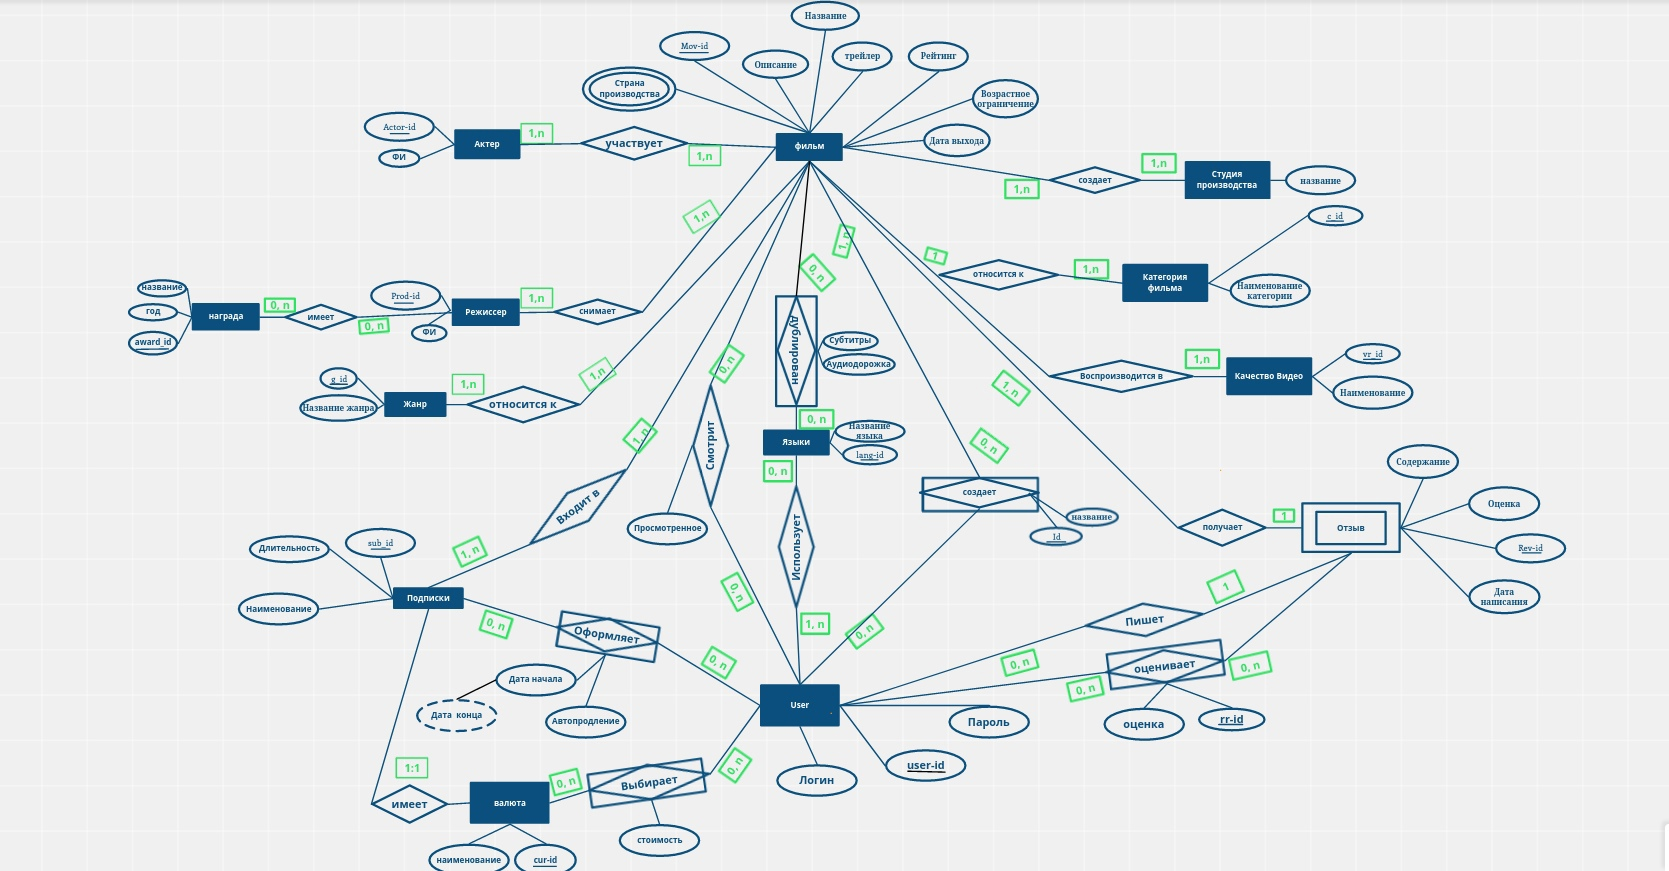
\includegraphics[width=1\linewidth]{concept}}
    \caption{Концептуальная модель базы данных}
\end{figure}

\subsection{Описание атрибутов}
\begin{thebibliography}{}

\end{thebibliography}


\end{document}
